%%%%%%%%%%%%%%%%%%%%%%%%%%%%%%%%%%%%%%%%%
% FAIMS3 Presentations
% LaTeX Template
% Version 1.0 (May 1, 2021)
%
% This template was created by:
% Vel (enquiries@latextypesetting.com)
% https://www.LaTeXTypesetting.com
%
%!TEX program = xelatex
% Note: this template must be compiled with XeLaTeX rather than PDFLaTeX
% due to the custom fonts used. The line above should ensure this happens
% automatically, but if it doesn't, your LaTeX editor should have a simple toggle
% to switch to using XeLaTeX.
%
%%%%%%%%%%%%%%%%%%%%%%%%%%%%%%%%%%%%%%%%%

\documentclass[
	aspectratio=169, % Wide slides by default
	11pt, % Default font size
	t, % Top align all slide content
]{beamer}

\usetheme{faims} % Use the FAIMS beamer theme
\usecolortheme{faims} % Use the FAIMS beamer color theme

\setbeamerfont{block title}{size=\scriptsize}
\setbeamerfont{block body}{size=\fontsize{5pt}{6pt}}
\bibliography{sample.bib} % BibLaTeX bibliography file

%----------------------------------------------------------------------------------------

\begin{document}

%----------------------------------------------------------------------------------------
%	 TITLE SLIDE
%----------------------------------------------------------------------------------------

\begin{titleframe} % Custom environment required for the title slide
	\frametitle{FAIMS 3.0 ARDC Platform Project}
	\framesubtitle{Annual Review: July 2020 to June 2021}

	Shawn Ross, Penny Crook and \newline
	Brian Ballsun-Stanton

	\vfill

 	\today

\end{titleframe}

%----------------------------------------------------------------------------------------
%	TABLE OF CONTENTS
%----------------------------------------------------------------------------------------

%\begin{frame}
%	\frametitle{Table of Contents}
%	\framesubtitle{One Column}
%
%	\tableofcontents % Sections are automatically populated from \section{} commands through the presentation
%\end{frame}

%------------------------------------------------

 \begin{frame}
     \frametitle{Table of Contents}
 %	\framesubtitle{Two Columns}

     \begin{columns}[t]
         \begin{column}{0.45\textwidth}
             \tableofcontents[sections={1-3}] % Sections are automatically populated from \section{} commands through the presentation
         \end{column}
         \hfill
         \begin{column}{0.45\textwidth}
             \tableofcontents[sections={4-6}] % Sections are automatically populated from \section{} commands through the presentation
         \end{column}
     \end{columns}
 \end{frame}

%----------------------------------------------------------------------------------------
\section{Overview}
\begin{sectionframe} % Custom environment required for section slides
	\frametitle{Overview}
	\framesubtitle{}

    \begin{columns}[t]
    \begin{column}{0.8\textwidth}
    {\color{faimsblue}\OpenSans\small
	This is a brief report to outline the progress we have made on the \textbf{FAIMS 3.0: Electronic Field Notebooks} project in our first year. It covers activities from July 2020 to June 2021.
	
	\medskip
	
    If you have any queries please contact us at \textbf{shawn@faims.edu.au} or \textbf{penny@faims.edu.au}.
    }
    \end{column}
    \begin{column}{0.15\textwidth}
    \end{column}
    \end{columns}

\end{sectionframe}

% %----------------------------------------------------------------------------------------

% \section{Text Examples}

% %----------------------------------------------------------------------------------------
% %	AUTOMATIC TEXT WRAPPING
% %----------------------------------------------------------------------------------------

% \begin{frame}[allowframebreaks] % 'allowframebreaks' allows automatic splitting across slides if the content is too long
% 	\frametitle{Automatic Text Wrapping}
% 	\framesubtitle{This text will automatically span across multiple slides\ldots}
	
% 	Lorem ipsum dolor sit amet, consectetur adipiscing elit. Praesent porttitor arcu luctus, imperdiet urna iaculis, mattis eros. Pellentesque iaculis odio vel nisl ullamcorper, nec faucibus ipsum molestie. Sed dictum nisl non aliquet porttitor.
	
% 	\bigskip
	
% 	Aliquam arcu turpis, ultrices sed luctus ac, vehicula id metus. Morbi eu feugiat velit, et tempus augue. Proin ac mattis tortor. Donec tincidunt, ante rhoncus luctus semper, arcu lorem lobortis justo, nec convallis ante quam quis lectus. Donec cursus maximus luctus. Vivamus lobortis eros et massa porta porttitor.

% 	\bigskip

% 	Fusce varius orci ac magna dapibus porttitor. In tempor leo a neque bibendum sollicitudin. Nulla pretium fermentum nisi, eget sodales magna facilisis eu. Praesent aliquet nulla ut bibendum lacinia.

% 	\bigskip

% 	Pellentesque lobortis justo enim, a condimentum massa tempor eu. Ut quis nulla a quam pretium eleifend nec eu nisl. Nam cursus porttitor eros, sed luctus ligula convallis quis. Nam convallis, ligula in auctor euismod, ligula mauris fringilla tellus, et egestas mauris odio eget diam. Praesent sodales in ipsum eu dictum.
% \end{frame}

% %----------------------------------------------------------------------------------------
% %	Admin Overview: 1 min
% %---------------------------------------------------------

\section{Project Administration}

\begin{frame}%[allowframebreaks]
	\frametitle{Project Administration}
    %\framesubtitle{}
    \textbf{The FAIMS3 Project:}
    
    \begin{itemize}
        \item was established in \textbf{June 2020} with a \$600,000 investment from the \href{https://ardc.edu.au/project/faims-3-0-electronic-field-notebooks/}{Australian Research Data Commons (ARDC)} and \$720,920 co-investment from project partners; 
        \item is hosted by Macquarie University; and supported by 39 participants from 23 universities and institutions; 
        \item is governed by a Leadership Team with oversight from a Steering Committee, Technical Advisory Group and Business Advisory Group.
 
    \end{itemize}
    
\textbf{Development team:}   
    
    \begin{itemize}
        \item Lead developers \href{https://www.aao.gov.au/}{Australian Astronomical Optics} (AAO Macquarie, formerly the Australian Astronomical Observatory)
        \item \href{https://www.csiro.au/en/about/people/business-units/mineral-resources}{ CSIRO Mineral Resources} (Perth, WA) leads QA testing architecture.
        \item AARnet leads development of integration services. 

    \end{itemize}

A Memorandum of Understanding between FAIMS, AAO and CSIRO governs all development activities. (An MoU with AARnet is in draft.)  



\end{frame} 

% %----------------------------------------------------------------------------------------
% %	Technical Overview: 4-5 min
% %----------------------------------------------------------------------------------------

\section{Technical Overview}


\begin{frame}%[allowframebreaks]
	\frametitle{Technical Overview}
    \framesubtitle{Design Goals}
    %\vspace{-.5cm}
    \textbf{FAIMS3} is a ground-up rewrite of the \href{https://github.com/FAIMS}{FAIMS Mobile (v2.6)} offline-capable, geospatial, multimedia, field-data collection application %\parencite{Ross2013-hi,Ross2015-ph, Sobotkova2015-lq, Sobotkova2016-mx, Ballsun-Stanton2018-zd, Sobotkova2018-al, VanValkenburgh2018-hv, Sobotkova2021-ms}
    . This rewrite is designed to be multi-platform, maintainable, and to support data collection at a citizen-science scale. The code and platform should last for at least five years, assuming regular maintenance.  Specifically \textbf{FAIMS3} will:
    
    \begin{itemize}
        \item Replicate all\textbf{ FAIMS v2.6} features that are currently used as part of three projects' research practice: CSIRO environmental geochemistry, LTU Mungo Lakes archaeology and UNSW Oral History. 
        \item Allow \textbf{self-service} customisation and deployment via a web application without needing FAIMS team intervention for the vast majority of deployments.
        \item Operate \textbf{cross-platform}, running the same code on Android, iOS, and `desktop'.
        \item Allow data \textbf{'round trip'} to web and desktop applications (ie data captured in-field, edited externally, can be returned to the device in editable format).
        \item \textbf{Improve} scalability and performance. Our target is ten times the number of records per deployment compared to v2.6 plus server-to-server synchronisation. 
     \end{itemize}
     \medskip
\end{frame} 

     
\begin{frame}
    \frametitle{Technical Overview}
    \framesubtitle{Development Progress}        
        \begin{itemize}
            \item The  \href{https://docs.google.com/document/d/13eTN8jhJa3Pgs9GOdo7r4jtIQcskNo7ikxJcBDBKHzw/edit}{FAIMS3 Technical Elaboration Report} was approved in February. This established the proof-of-concept for FAIMS3. 
          \item The FAIMS3 \href{https://github.com/FAIMS/FAIMS3/releases/tag/v0.1.0-alpha}{Alpha prototype} was released on 11 June 2021.  
          \item The FAIMS3 Alpha prototype passed \href{https://doi.org/10.5281/zenodo.5030772}{user-acceptance testing} on 15 June 2021 (see next slide).
        \item FAIMS3 code has been licensed under the \href{https://www.apache.org/licenses/LICENSE-2.0}{Apache2} license, a Developer Contribution agreement is being applied to all code affirming the license. 
        \item The FAIMS3 repository is now public on \href{https://github.com/FAIMS/FAIMS3}{GitHub}.
        \item FAIMS3 Beta development commenced on 5 July 2021. 

    \end{itemize}



\end{frame} 


% To not have this automatically overflow use:
% \begin{frame}
% frame means "slide"
% Otherwise use:
% \begin{frame}%[allowframebreaks]
% 	\frametitle{Development}
%     \framesubtitle{Completed Activities}
%     Key developments since last Update:
    
%     \begin{itemize}
%         \item Our FAIMS 2.6 servers were migrated to AAO hardware. These servers will support the last of the FAIMS 2.6 projects as we await FAIMS 3. They were field tested in April for work in the Blue Mountains.
%         \item Acquired hardware (iPads and Chromebooks) for testing.

%     \end{itemize}
    
% Action items:    
    
%     \begin{itemize}
%         \item NA
%     \end{itemize}

% \end{frame}

% %----------------------------------------------------------------------------------------% %	


\begin{frame}
\frametitle{Technical Overview}
\framesubtitle{FAIMS3 Alpha Prototype}
\vspace{-.75cm}
\begin{columns}
\begin{column}{0.5\textwidth}

\medskip 

\textbf{FAIMS 3.0 has successfully deployed onto Google Chrome, Android, and iOS! } \medskip 

The goals of Alpha prototype were: \smallskip

`\textit{To demonstrate the foundational capabilities of FAIMS3. Specifically, loading a module from a specification file, data entry on all OSes, and asynchronous data exchange on an append-only datastore.}' \medskip 

For more information see the \href{https://doi.org/10.5281/zenodo.5030772}{UAT report}. \smallskip 

End-to-end test demonstrations of Alpha on \href{https://youtu.be/79_sIVg8zDM}{Android} and \href{https://youtu.be/O4btmhKLyc4}{web browser} are on the FAIMS Project's YouTube channel.  

\end{column}
\begin{column}{0.2\textwidth}
\begin{center}
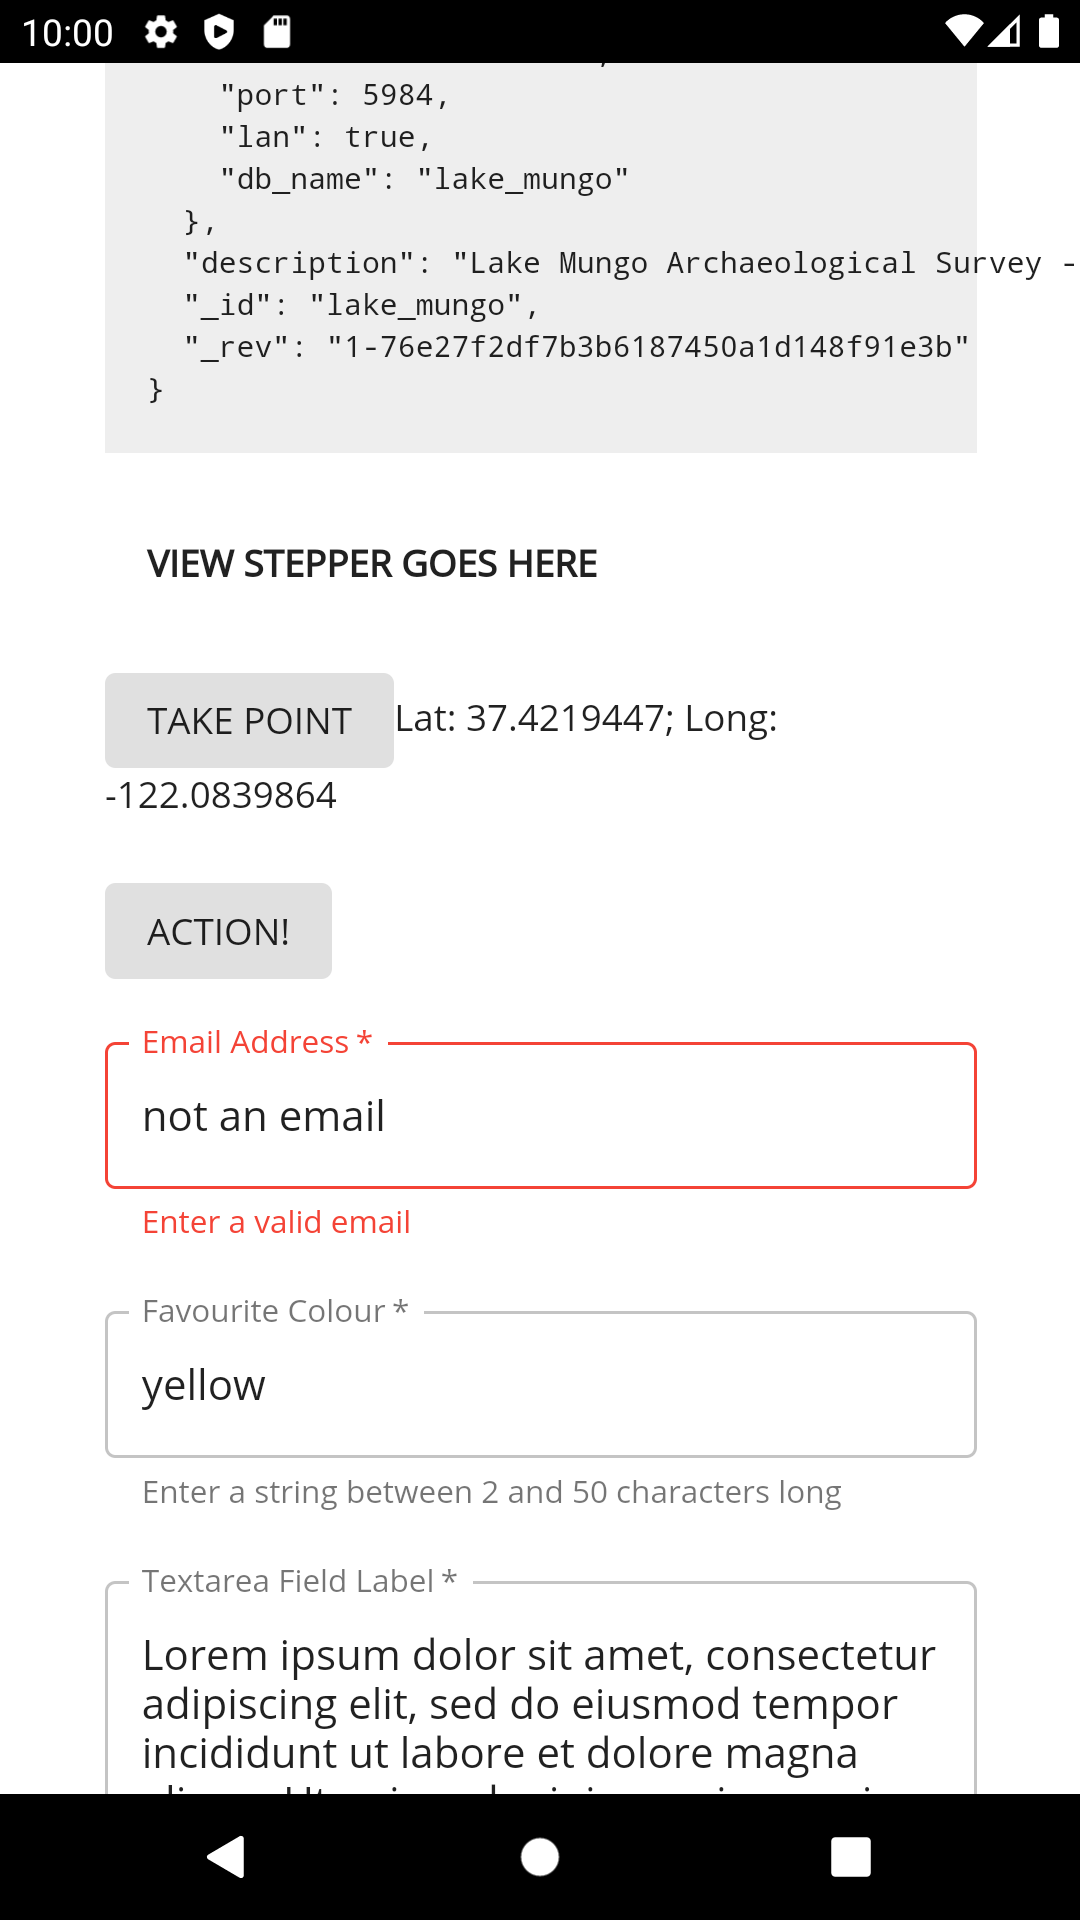
\includegraphics[width=\textwidth]{Images/Screenshot_1620777635.png}
\end{center}
\end{column}
\begin{column}{0.17\textwidth}
\begin{center}
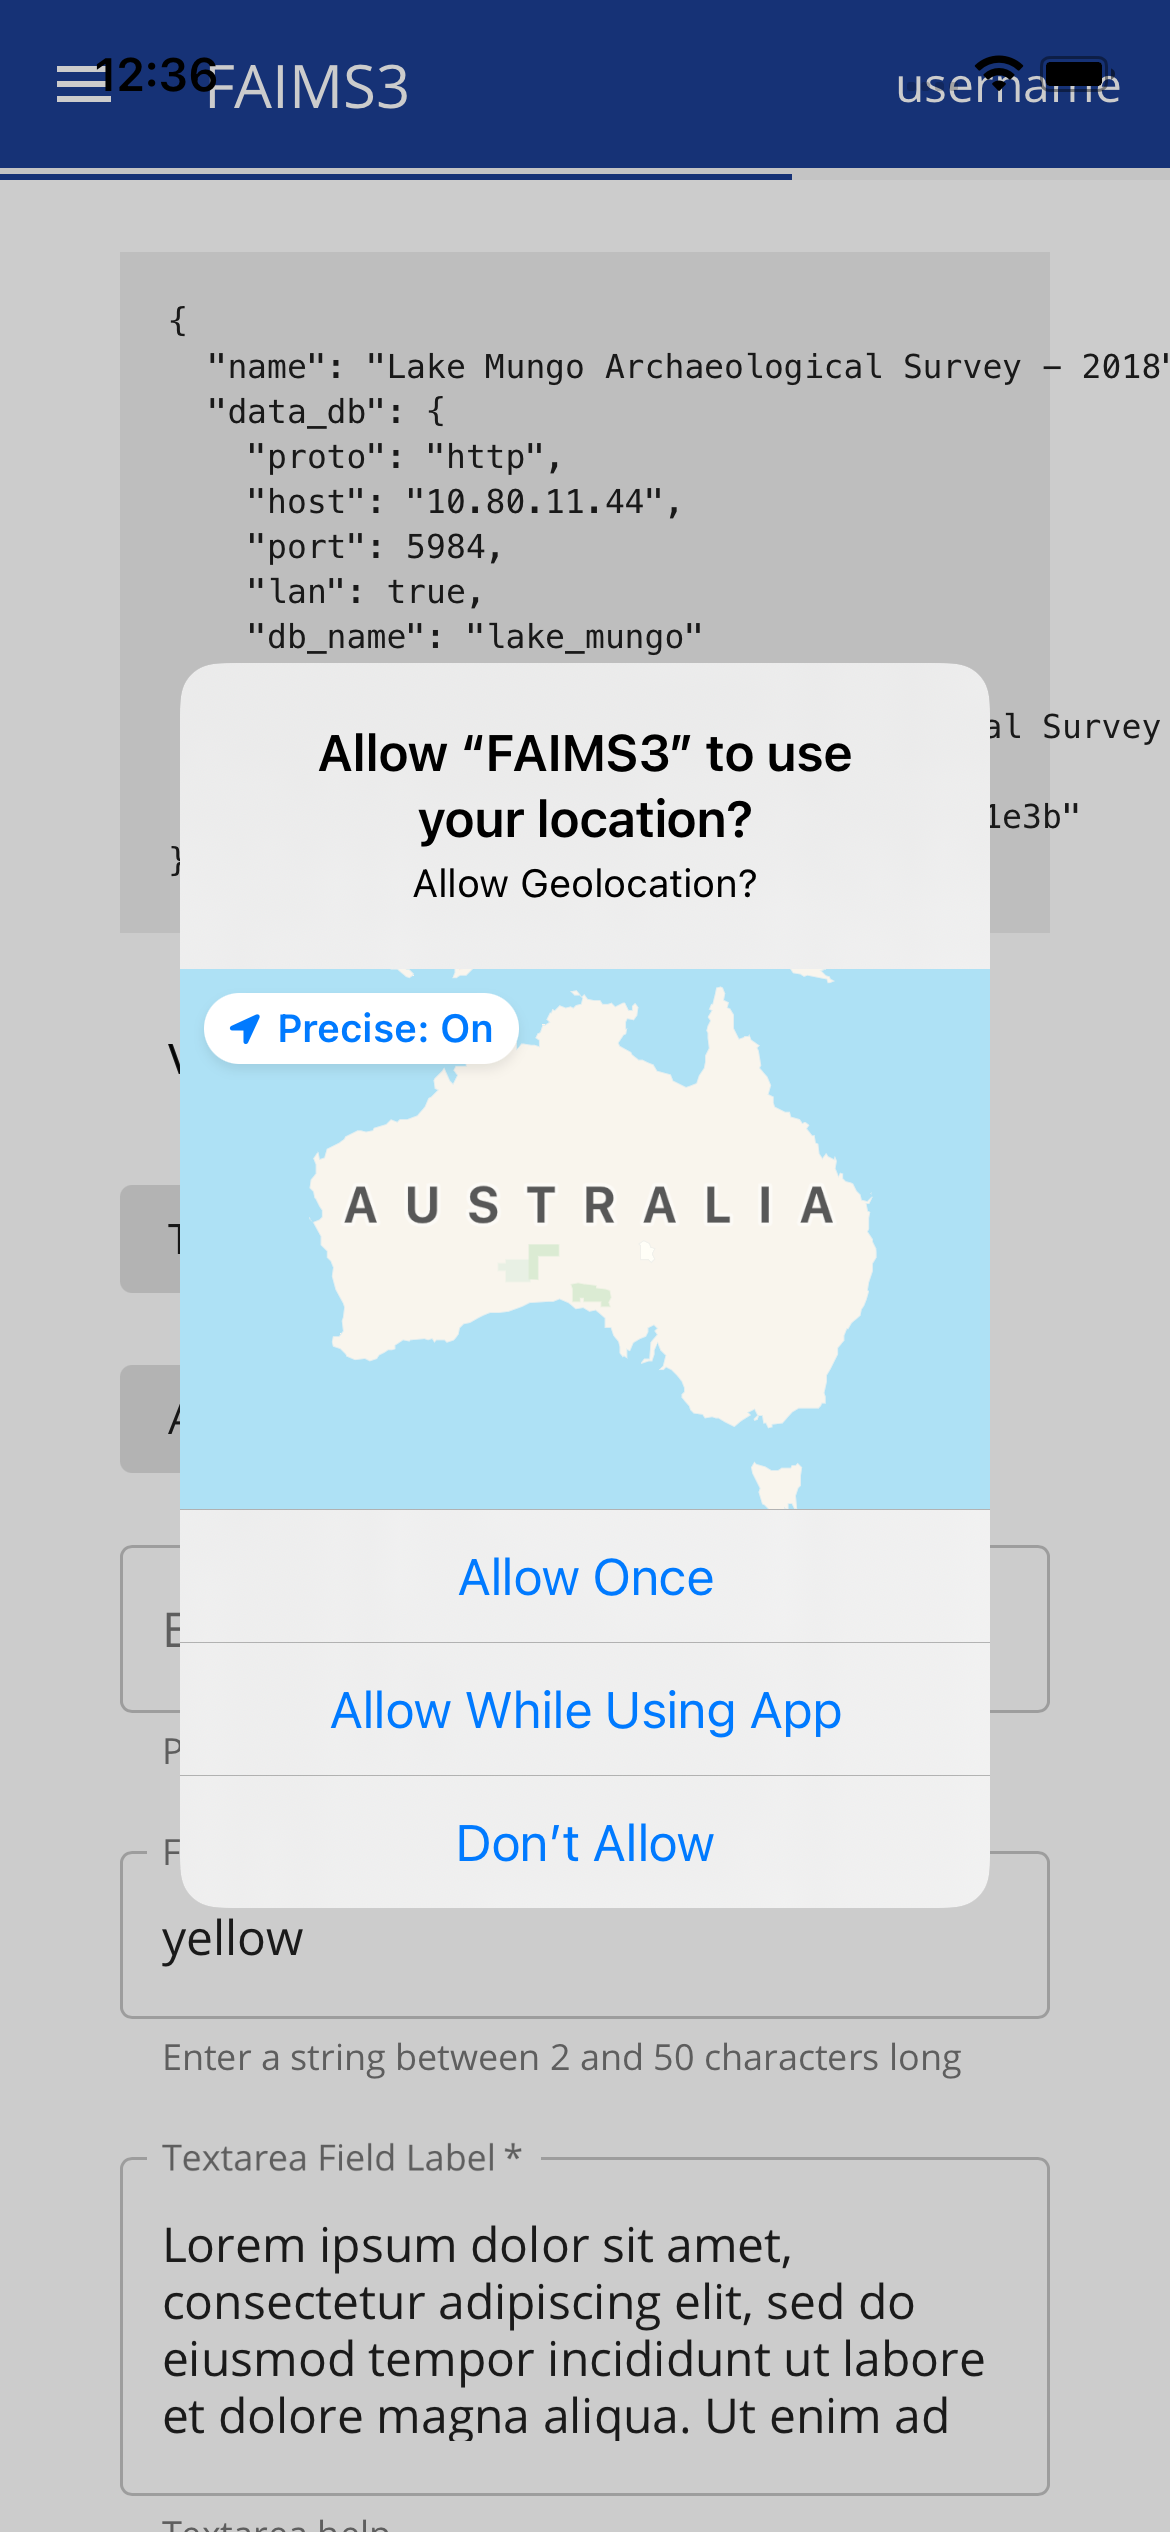
\includegraphics[width=\textwidth]{Images/Simulator Screen Shot - iPhone 12 - 2021-05-12 at 12.36.55.png}
\end{center}
\end{column}
\end{columns}
\end{frame}

% %----------------------------------------------------------------------------------------
% %	Outreach and Engagement: 3 min
% %---------------------------------------------------------

\section{Outreach and Engagement}

\begin{frame}%[allowframebreaks]
	\frametitle{Outreach and Engagement}
    % \framesubtitle{}
    In our first year the FAIMS3 project has:
    \begin{itemize}
        \item Refreshed our branding package
        \item established a \href{https://faims.edu.au/}{website}, \href{https://faims.substack.com}{Newsletter}, \href{https://osf.io/mqk45/}{OSF page} and \href{https://zenodo.org/communities/faims/}{Zenodo community} 
        \item delivered 13 seminars and presentations (by leadership and project partners)
        \item prepared 3 newsletter blog posts
        \item submitted one paper for publication
        \item partnered with another ARDC Platform project: \href{https://doi.org/10.47486/PL005}{AgReFed: A platform for the transformation of agricultural research} led by Federation University to improve data collection and dissemination for agricultural researchers
        \end{itemize}
    
    \medskip
    
   A list of seminars and outputs are listed at the end of this slide deck. 

\end{frame}

% \begin{frame}%[allowframebreaks]
% 	\frametitle{Activities in Progress}
%     \framesubtitle{Development}
%     We are working on:
    
%     \begin{itemize}
%         \item Development of the \textbf{alpha prototype} (Milestone 4.3). AAO developers are committing code and CSIRO has been developing testing pipelines. Alpha will be a demonstration of the core capacity of FAIMS3: offline, multi-user, cross-platform data collection. Specifically, the goal of alpha is `To demonstrate the foundational capabilities of FAIMS3. Specifically, loading a module from a specification file, data entry on all OSes, and asynchronous data exchange on an append-only datastore, plus demonstrating whatever authentication mechanisms we have implemented'. Alpha is expected to be ready at the end of May and ready for user-acceptance testing in June.
%         \item Planning for \textbf{outreach activities} for the alpha release in collaboration with Luc Betbeder-Matibet and David Jung from UNSW. A Communications Roadmap will be developed in May and June.
%         \item We continue to work on \textbf{updating the website} to retire FAIMS 2.6 information and introduce FAIMS3. 
%         \item Archive FAIMS reports, outputs, etc., from 2012 to 2019 (in Zenodo and OSF). 
        
%     \end{itemize}
    
%     Action items:
    
%     \begin{itemize}
%     \item NA
%     \end{itemize}
    

% \end{frame}


% %----------------------------------------------------------------------------------------
% %	Technical Overview: 3 min
% %-----------------------------------------------------


\section{Commercialisation}


\begin{frame}%[allowframebreaks]
	\frametitle{Commercialisation}
    % \framesubtitle{}
   The long-term maintenance of FAIMS3 will be supported by a Commercial Open Source Software (COSS) model: a self-service, open-source core with value-added services to generate revenue to share the cost of updates, upgrades and feature development. While no commercial services will be offered until 2023, in our first year we have conducted the following     \textbf{commercialisation activities:}
    
    \begin{itemize}
        \item With assistance from CSIRO ON and Elevate legal, members of the FAIMS3 Leadership team established a company to provide services around the software we develop: \textbf{Electronic Field Notebooks Pty Ltd}. Shawn Ross is the company director. 
        \item Commenced negotiation with \textbf{MQ Commercialisation} to enter a partnership with EFN, clarifying IP arrangements and providing ongoing support for COSS model.
        \item A draft \textbf{Business Plan} was endorsed by the Business Advisory Group in May 2021. It will remain a working document throughout our development and will be revised in May 2022 (following the first report on the Beta field deployments) and again in February 2023. 
        

    \end{itemize}
    
  

\end{frame}

\section{Outputs}

\begin{frame}[allowframebreaks]
	\frametitle{Outputs}
    %\framesubtitle{Presentations}
    
    \textbf{Publications and Preprints}
    \begin{enumerate}
    \item Ross, S.A. and B. Ballsun-Stanton. 2022. `Introducing Preregistration of Research Design to Archaeology', in E. Watrall and L. Goldstein (ed.) \textit{Digital Heritage and Archaeology in Practice}. Gainesville, FL: University Press of Florida. (See  \href{https://osf.io/preprints/socarxiv/sbwcq}{SocARXIV} )
    \end{enumerate}
    
    \textbf{Digital Media}
    \begin{enumerate}
    \item  FAIMS was selected as a case study for the ARDC website: \href{https://ardc.edu.au/about_us/case-studies/dirt-to-desktop-digital-tools-in-the-field/}{Dirt to desktop: Digital tools in the field}, June 2021.
    \end{enumerate}
    \textbf{Presentations}
        \begin{enumerate}
            \item SA Ross, ‘Eight Years of FAIMS Mobile: Reflecting Backward, Looking Ahead’, UTS Digital Histories research seminar, 14 May 2020.
            \item SA Ross, ‘FAIMS 3.0 project’, Introduction to the First Round of Platforms Projects, ARDC webinar, 24 June 2020. 
            \item SA Ross, B Ballsun-Stanton, S Cassidy, P Crook, A Sobotkova and J Klump, `\href{https://github.com/saross/FAIMS-intro/releases/tag/v3.0}{FAIMS 3.0: Electronic Field Notebooks}', Session 3: Data Management, Computer Applications in Archaeology Australasia Online Conference, 11 September 2020.
               \item A Sobotkova and P Crook ‘Research Data Management (RDM) services’, Research Data Alliance workshop, 5 November 2020. (See \href{https://wiki.geant.org/display/EV/RDM-Services}{RDM Services})
	        \item E K Bone, Gray A. Williams, and Bayden D. Russell, ‘Creating a Digital Learning Ecosystem to Facilitate Authentic Place-Based Learning and International Collaboration: A Coastal Case Study’, ASCILITE 2020 Conference Online, hosted by UNE, 30 November 2020.
            \item A Sobotkova Digital Data Collection in Archaeology, Seminar at Department of Archaeology, Aarhus University convened by Jens Andersen, 23 April 2020.
            \item Simons, N., Clark, J., Brown, J., Gould, M., Lannom, L., Vials Moore, A., et al. (2020, November). PIDs: Joining up the World - PID IG at RDA P16 2020. Conference Presentation presented at the Research Data Alliance Plenary 16 (RDA), Costa Rica (Virtual). (See \href{https://doi.org/10.5281/zenodo.4291878}{Zenodo}.)
            \item J Klump, ARDC seminar on IGSN, the Australian perspective, 30 March 2020.
            \item J Klump, Presentation to the USGS on IGSN, 02 April 2020.
            \item A Sobotkova, ‘FAIMS 3.0: Electronic Field Notebooks: Human-Mediated Field Data Collection’, GeoConvergence Workshop: An event by the American Geographical Society in support of the National Science Foundation, 19 May 2021. (See \href{https://www.geoconvergence.org/ltblog/sobotkova}{www.geoconvergence.org} or \href{https://osf.io/k7c5h/}{OSF}.)
            \item Lesley Wyborn (NCI, ANU), introduced FAIMS to a meeting of researchers and government agencies on Geophysical data standards, 25 March 2021. A short Introduction to FAIMS was prepared and is accessible at https://osf.io/f9hqw/. 
            \item A Sobotkova and P. Hermankova, 'Good digital tools do not make or break field survey...but they sure help!', CAA 2021 Virtual Limassol, 17 June 2021. (See \href{https://2021.caaconference.org/sessions/\#1}{S1 Roundtable}) 
            \item N Buławka, J M Chyla, G P Cirigliano and A Sobotkova 'Documenting the shift in mound condition measurement at a long-term archaeological project', CAA 2021 Virtual Limassol, 17 June 2021. (See  \href{https://2021.caaconference.org/sessions/\#22}{S22})

    \end{enumerate}

\end{frame}


%\section{Project Information}






% %----------------------------------------------------------------------------------------
% % FONT OPTIONS
% %----------------------------------------------------------------------------------------

% \begin{frame}
% 	\frametitle{Font Options}

% 	Open Sans Light (default): Light, \textbf{Semibold}, \textit{LightItalic}, \textbf{\textit{SemiboldItalic}}

% 	\medskip

% 	Open Sans: {\OpenSans Regular, \textbf{Bold}, \textit{Italic}, \textbf{\textit{BoldItalic}}}

% 	\medskip

% 	Open Sans Condensed: {\OpenSansCondensed CondensedLight, \textbf{CondensedBold}, \textit{CondensedLightItalic}}

% 	\bigskip

% 	{\tiny tiny} {\scriptsize scriptsize} {\footnotesize footnotesize} {\small small} {\normalsize normalsize} {\large large} {\Large Large} {\LARGE LARGE} {\huge huge}
% \end{frame}

% %----------------------------------------------------------------------------------------
% %	SLIDE WITHOUT TITLE
% %----------------------------------------------------------------------------------------

% \begin{frame}
% 	Slides don't need to have titles.
% \end{frame}

% %----------------------------------------------------------------------------------------
% %	SLIDE WITHOUT TITLE WITH TITLE PADDING
% %----------------------------------------------------------------------------------------

% \begin{frame}
% 	\frametitle{\empty} % Empty so vertical whitespace is still added

% 	Slides can have empty titles, for alignment of content with slides with titles.
% \end{frame}

% %----------------------------------------------------------------------------------------
% %	EMPTY NO PADDING SLIDE
% %----------------------------------------------------------------------------------------

% \begin{frame}[plain]
% 	Slides can also be completely plain with no headers/footers and padding.

% 	\bigskip

% 	This is useful for large tables or figures.
% \end{frame}

% %----------------------------------------------------------------------------------------
% %	SECTION HIERARCHY
% %----------------------------------------------------------------------------------------

% \begin{frame}
% 	\frametitle{Heading Styling}

% 	\headinglevelone{Heading Level 1}

% 	Lorem ipsum dolor sit amet, consectetur adipiscing elit. Morbi eu feugiat velit, et tempus augue.
	
% 	\headingleveltwo{Heading Level 2}

% 	Praesent porttitor arcu luctus, imperdiet urna iaculis, mattis eros. Pellentesque iaculis odio vel nisl ullamcorper, nec faucibus ipsum molestie.
	
% 	\headinglevelthree{Heading Level 3}

% 	Sed dictum nisl non aliquet porttitor.
% \end{frame}

% %----------------------------------------------------------------------------------------

% \section{Blocks and column examples}

% %----------------------------------------------------------------------------------------
% %	COLUMNS
% %----------------------------------------------------------------------------------------

% \begin{frame}
% 	\frametitle{Using Columns}
% 	\framesubtitle{Two Columns}

% 	\begin{columns}[T]
% 		\begin{column}{0.45\textwidth}
% 			Lorem ipsum dolor sit amet, consectetur adipiscing elit. Morbi eu feugiat velit, et tempus augue. Praesent porttitor arcu luctus, imperdiet urna iaculis, mattis eros. Pellentesque iaculis odio vel nisl ullamcorper, nec faucibus ipsum molestie. Sed dictum nisl non aliquet porttitor.
% 		\end{column}
		
% 		\hfill

% 		\begin{column}{0.45\textwidth}
% 			Etiam vulputate arcu dignissim, finibus sem et, viverra nisl. Aenean luctus congue massa, ut laoreet metus ornare in. Nunc fermentum nisi imperdiet lectus tincidunt vestibulum at ac elit. Nulla mattis nisl eu malesuada suscipit.
% 		\end{column}
% 	\end{columns}
% \end{frame}

% %------------------------------------------------

% \begin{frame}
% 	\frametitle{Using Columns}
% 	\framesubtitle{Three Columns}

% 	\begin{columns}[T]
% 		\begin{column}{0.3\textwidth}
% 			Lorem ipsum dolor sit amet, consectetur adipiscing elit. Praesent porttitor arcu luctus, imperdiet urna iaculis, mattis eros. Pellentesque iaculis odio vel nisl ullamcorper.
% 		\end{column}

% 		\begin{column}{0.3\textwidth}
% 			
\includegraphics[width=\textwidth]{Faims-large.png}\\[6pt]
% 			Aenean tincidunt sodales massa, et hendrerit tellus mattis ac.
% 		\end{column}
		
% 		\begin{column}{0.3\textwidth}
% 			Aliquam arcu turpis, ultrices sed luctus ac, vehicula id metus. Morbi eu feugiat velit, et tempus augue. Proin ac mattis tortor. Donec tincidunt, ante rhoncus luctus semper.
% 		\end{column}
% 	\end{columns}
% \end{frame}

% %----------------------------------------------------------------------------------------
% %	BLOCKS
% %----------------------------------------------------------------------------------------

% \begin{frame}
% 	\frametitle{Using Beamer Blocks}

% 	\begin{columns}[T]
% 		\begin{column}{0.3\textwidth}
% 			\begin{block}{Block Title}
% 				Aliquam arcu neque, ornare in, ullamcorper quis, commodo eu, libero. Maecenas sapien libero, lobortis in, sodales eget, dui.
% 			\end{block}
% 		\end{column}

% 		\begin{column}{0.3\textwidth}
% 			\begin{block}{\centering Centered Block Title}
% 				Aliquam arcu neque, ornare in, ullamcorper quis, commodo eu, libero. Maecenas sapien libero, lobortis in, sodales eget, dui.
% 			\end{block}
% 		\end{column}

% 		\begin{column}{0.3\textwidth}
% 			\begin{block}{\vspace{-\baselineskip}}
% 				Aliquam arcu neque, ornare in, ullamcorper quis, commodo eu, libero. Maecenas sapien libero, lobortis in, sodales eget, dui.
% 			\end{block}
% 		\end{column}
% 	\end{columns}
% \end{frame}

% %----------------------------------------------------------------------------------------
% %	ALERT BLOCK
% %----------------------------------------------------------------------------------------

% \begin{frame}
% 	\frametitle{Alert Blocks}
% 	\framesubtitle{Useful for Important Information}

% 	\begin{columns}[T]
% 		\begin{column}{0.45\textwidth}
% 			Etiam vulputate arcu dignissim, finibus sem et, viverra nisl. Aenean luctus congue massa, ut laoreet metus ornare in. Nunc fermentum nisi imperdiet lectus tincidunt vestibulum at ac elit. Nulla mattis nisl eu malesuada suscipit.
% 		\end{column}
		
% 		\hfill

% 		\begin{column}{0.45\textwidth}
% 			\vspace*{-\baselineskip} % For vertical alignment with the text
% 			\begin{alertblock}{Alert Block Title}
% 				Suspendisse vitae elit. Aliquam arcu neque, ornare in, ullamcorper quis, commodo eu, libero. Fusce sagittis erat at erat tristique mollis. Maecenas sapien libero, molestie et, lobortis in, sodales eget, dui.
% 			\end{alertblock}
% 		\end{column}
% 	\end{columns}
% \end{frame}

% %----------------------------------------------------------------------------------------
% %	EXAMPLE BLOCK
% %----------------------------------------------------------------------------------------

% \begin{frame}
% 	\frametitle{Example Blocks}

% 	\begin{columns}[T]
% 		\begin{column}{0.6\textwidth}
% 			\vspace*{-\baselineskip} % For vertical alignment with the text
% 			\begin{exampleblock}{Example Block Title}
% 				Suspendisse vitae elit. Aliquam arcu neque, ornare in, ullamcorper quis, commodo eu, libero. Fusce sagittis erat at erat tristique mollis. Maecenas sapien libero, molestie et, lobortis in, sodales eget, dui. Morbi ultrices rutrum lorem. Nam elementum ullamcorper leo. Morbi dui. Aliquam sagittis. Nunc placerat. Pellentesque tristique sodales est.
% 			\end{exampleblock}
% 		\end{column}

% 		\hfill

% 		\begin{column}{0.3\textwidth}
% 			Etiam vulputate arcu dignissim, finibus sem et, viverra nisl. Aenean luctus congue massa, ut laoreet metus ornare in. Nunc fermentum nisi imperdiet lectus tincidunt vestibulum at ac elit.
% 		\end{column}
% 	\end{columns}
% \end{frame}

% %----------------------------------------------------------------------------------------

% \section{Slide element examples}

% %----------------------------------------------------------------------------------------
% %	LISTS
% %----------------------------------------------------------------------------------------

% \begin{frame}
% 	\frametitle{Lists}

% 	\begin{enumerate}
% 		\item First numbered item
% 		\begin{enumerate}
% 			\item First indented numbered item
% 			\item Second indented numbered item
% 			\begin{enumerate}
% 				\item First second-level indented numbered item
% 			\end{enumerate}
% 		\end{enumerate}
% 		\item Second numbered item
% 	\end{enumerate}

% 	\rule{\textwidth}{0.25pt}

% 	\begin{itemize}
% 		\item First bullet point item
% 		\begin{itemize}
% 			\item First indented bullet point item
% 			\item Second indented bullet point item
% 			\begin{itemize}
% 				\item First second-level indented bullet point item
% 			\end{itemize}
% 		\end{itemize}
% 		\item Second bullet point item
% 	\end{itemize}
% \end{frame}

% %----------------------------------------------------------------------------------------
% %	TABLE
% %----------------------------------------------------------------------------------------

% \begin{frame}
% 	\frametitle{Table}
% 	\framesubtitle{Displaying Data}

% 	\begin{table}
% 		\centering % Center the table in the slide
% 		\begin{tabular}{L{0.18\textwidth} R{0.11\textwidth} R{0.11\textwidth}}
% 			\toprule
% 			\textit{Per 50g} & \textbf{Pork} & \textbf{Soy} \\
% 			\midrule
% 			Energy & 760kJ & 538kJ\\
% 			Protein & 7.0g & 9.3g\\
% 			Carbohydrate & 0.0g & 4.9g\\
% 			Fat & 16.8g & 9.1g\\
% 			Sodium & 0.4g & 0.4g\\
% 			Fibre & 0.0g & 1.4g\\
% 			\bottomrule
% 		\end{tabular}
% 	\end{table}
% \end{frame}

% %----------------------------------------------------------------------------------------
% %	IMAGE
% %----------------------------------------------------------------------------------------

% \begin{frame}
% 	\frametitle{Image/Figure}
% 	\framesubtitle{Including a Centered Image, Such As of a Graphical Figure}

% 	\begin{center}
% 		
\includegraphics[width=0.5\textwidth]{Faims-large.png}
% 	\end{center}
% \end{frame}

% %----------------------------------------------------------------------------------------
% %	EQUATION
% %----------------------------------------------------------------------------------------

% \begin{frame}
% 	\frametitle{Equation}

% 	\begin{equation}
% 		\cos^3 \theta =\frac{1}{4}\cos\theta+\frac{3}{4}\cos 3\theta
% 	\end{equation}
% \end{frame}

% %----------------------------------------------------------------------------------------
% %	REFERENCES
% %----------------------------------------------------------------------------------------

% \begin{frame}
% 	\frametitle{Referencing}

% 	This statement requires citation \autocite{Smith:2019qr}. This statement requires multiple citations \autocite{Smith:2019qr, Smith:2021jd}. This statement contains an in-text citation, reminiscent of that in \textcite{Smith:2021jd}.
% \end{frame}

% %----------------------------------------------------------------------------------------

% \section{Custom slides}

% %----------------------------------------------------------------------------------------
% %	IMAGE SLIDE
% %----------------------------------------------------------------------------------------

% \imageslide{Monasterio_Khor_Virap_Armenia.jpg} % Image automatically takes up the full width of the slide, crop it if it's too tall

% %----------------------------------------------------------------------------------------
% %	BIG NUMBER SLIDE
% %----------------------------------------------------------------------------------------

% \begin{bignumframe}{20\%} % Big number slide, first argument should be the big number
% 	Lorem ipsum dolor sit amet, consectetur adipiscing elit. Praesent porttitor arcu luctus, imperdiet urna iaculis, mattis eros.

% 	\bigskip

% 	\begin{itemize}
% 		\item Etiam vulputate arcu dignissim, finibus sem et, viverra nisl.
% 		\item Aenean luctus congue massa, ut laoreet metus ornare in.
% 	\end{itemize}
% \end{bignumframe}

% %----------------------------------------------------------------------------------------
% %	REFERENCE LIST
% %----------------------------------------------------------------------------------------

% \begin{frame}[allowframebreaks] % 'allowframebreaks' allows automatic splitting across slides if the content is too long
% 	\frametitle{Bibliography}

% 	\printbibliography[heading=none]
% \end{frame}

% %----------------------------------------------------------------------------------------

% Long section title example

% \section{Project Governance}


% \begin{frame}
% 	\frametitle{FAIMS3 Project Governance}
% 	\vspace{-.5cm}
% \begin{columns}[T]
% \begin{column}{\textwidth}
%     \begin{block}{\vspace{-\baselineskip}}
% {\color{faimsblue}\textbf{Steering Committee}}\newline
% {\textbf{Composition:}  Participants named on application who are not part of the Leadership Team, or nominated replacement (\href{https://drive.google.com/a/fedarch.org/open?id=1_MER0X1HHTUfswwiWXR34yxf44OIofk0hbby34YI5_k}{participant list}). 
% \newline
% \textbf{Role:} (1) Review brief monthly reports on progress. (2) Confirm and approve completion of milestones. (3) Nominate (self or others) to groups / panels below as necessary (incl. UAT). Workload will be light and focused on higher-level governance - ensuring the overall project is on track.}
% 			\end{block}
% \end{column}\end{columns}
% 	\begin{columns}[T]
% 		\begin{column}{0.48\textwidth}
% 			\begin{block}{\vspace{-\baselineskip}}
% 			{\color{faimsblue}\textbf{Technical Advisory Group}}\newline
% 				\textbf{Composition}: See \href{https://drive.google.com/a/fedarch.org/open?id=1_MER0X1HHTUfswwiWXR34yxf44OIofk0hbby34YI5_k}{participant list}.  \textbf{Role}: Support Leadership Team in the development of a technical approach (typically selection of a preferred technology or pathway from among a finite list generated during technical elaboration by the Leadership Team and project staff). 
% 			\end{block}
% 		\end{column}
% 		\begin{column}{0.48\textwidth}
% 			\begin{block}{\vspace{-\baselineskip}}
% 			{\color{faimsblue}\textbf{Business Advisory Group}}\newline
% 				\textbf{Composition}: see \href{https://drive.google.com/a/fedarch.org/open?id=1_MER0X1HHTUfswwiWXR34yxf44OIofk0hbby34YI5_k}{participant list}. \newline \textbf{Role}: Support Leadership Team in the development of a business model / plan (including improvement of value propositions and business model canvas, review of financial model, formulation of product / service packages and pricing). 
% 			\end{block}
% 		\end{column}
% 	\end{columns}
% 	\begin{columns}[T]
% \begin{column}{\textwidth}
%     \begin{block}{\vspace{-\baselineskip}}
%     {\color{faimsblue}\textbf{Leadership Team}}\newline
%     \textbf{Composition}: Shawn Ross (MQ), Penny Crook (MQ), Jens Klump (CSIRO), Steve Cassidy (MQ), Brian Ballsun-Stanton (MQ), Adela Sobotkova (Aarhus). \newline
%     \textbf{Role}: Day-to-day operation of project. Management of project staff. Management of software development and QA / testing. Production of business plan. Communication and consultation with Steering Committee, Advisory Groups, and User Panels. Organisation of outreach and communication (including sales / marketing of any commercial product). Documented delivery of milestones.
% 			\end{block}
% \end{column}\end{columns}
% \begin{columns}[T]
% 		\begin{column}{0.48\textwidth}
% 			\begin{block}{\vspace{-\baselineskip}}
% 			{\color{faimsblue}\textbf{Ad hoc User Panels}}\newline
% 				\textbf{Composition}: drawn from / nominated by members of other committees. \newline
%                 \textbf{Role}: (1) Advising regarding the importance of software features / capabilities or palatability of business plan details. (2) User acceptance testing.
% 			\end{block}
% 		\end{column}
% 		\begin{column}{0.48\textwidth}
% 			\begin{block}{\vspace{-\baselineskip}}
% 			{\color{faimsblue}\textbf{Ad hoc User Panels}}\newline
% 					\textbf{Composition}: drawn from / nominated by members of other committees. \newline
%                 \textbf{Role}: (1) Advising regarding the importance of software features / capabilities or palatability of business plan details. (2) User acceptance testing.
% 			\end{block}
% 		\end{column}
% 	\end{columns}
% \end{frame}


% \begin{frame}
% 	\frametitle{FAIMS3 Development Organisation}
% %\begin{columns}[T]
% %\begin{column}{\textwidth}
% \begin{block}{Leadership Team}
% \textbf{Composition}: Shawn Ross (MQ), Penny Crook (MQ), Jens Klump (CSIRO), Steve Cassidy (MQ), Brian Ballsun-Stanton (MQ), Adela Sobotkova (Aarhus).
% \end{block}


% \vspace{-.5cm}
% %\end{column}\end{columns}
% %\begin{columns}[T]
% %\begin{column}{.3\textwidth}

% \begin{minipage}[t][.4\textheight][t]{.31\textwidth}
% \begin{block}{East Coast Development}
% \begin{minipage}[t][.4\textheight][t]{\textwidth}
% \textbf{Leaders}: Shawn Ross (MQ), Penny Crook (MQ), Steve Cassidy (MQ), Brian Ballsun-Stanton (MQ).\medskip

% \textbf{Budgeted project staff}: Development undertaken by AAO.\medskip

% \textbf{In-kind project staff}: Outreach and engagement (LTU \& UNSW)\medskip

% \textbf{Responsibilities}: Software development and documentation; integration of repositories; outreach and engagement.

% \end{minipage}
% \end{block}
% \end{minipage}
% \hfill
% %\end{column}
% %\begin{column}{.3\textwidth}
% \begin{minipage}[t][.4\textheight][t]{.31\textwidth}
% \begin{block}{West Coast Development}
% \begin{minipage}[t][.4\textheight][t]{\textwidth}

% \textbf{Leader}: Jens Klump (CSIRO).\medskip

% \textbf{Budgeted project staff}: Quality assurance lead, tester(s).\medskip

% \textbf{In-kind project staff}: Geosciences development; quality assurance and testing; CI / CD pipeline; outreach and engagement (CSIRO)\medskip

% \textbf{Responsibilities}: Quality assurance and testing; outreach and engagement.


% \end{minipage}
% \end{block}
% \end{minipage}
% %\end{column}
% %\begin{column}{.3\textwidth}
% \hfill
% \begin{minipage}[t][.4\textheight][t]{.31\textwidth}
% \begin{block}{Europe Development}
% \begin{minipage}[t][.4\textheight][t]{\textwidth}


% \textbf{Leaders}: Adela Sobotkova (Aarhus), Guido Aben (AARNet).\medskip

% \textbf{In-kind project staff}: Cloudstor development and documentation (AARNet); outreach and engagement (Aarhus)\medskip

% \textbf{Responsibilities}: Cloudstor integration; outreach and engagement with European organisations.
% \end{minipage}
% \end{block}
% \end{minipage}
% %\end{column}
% %\end{columns}
% \end{frame}

% ----------------------------------------------------------------------------------------
% 	CLOSING SLIDE
% ----------------------------------------------------------------------------------------

\closingslide % Output closing slide, automatically populated with a background image

----------------------------------------------------------------------------------------

\end{document}
